\documentclass[index]{subfiles}

\begin{document}

\begin{titlepage}
    \begin{center}
        \vspace*{1cm}

        {\huge{Testing the effective duration of the ATP-CP system}}

        \vspace{1.5cm}

        \vfill

        IB Sports Science SL Internal Assessment\\
        jkv635\\

    \end{center}
\end{titlepage}

\addtocontents{toc}{\protect\thispagestyle{empty}}
\tableofcontents
\thispagestyle{empty}
\newpage
\setcounter{page}{1}

\section{Introduction}

As both a current long-distance runner as well as a former sprinter, the question of when to transition from ``full-throttle'' to ``settling in'' in pace has always been on my mind whenever I start a race. When I learned about the different energy systems the body uses to supply muscles with energy during exercise in class, I wondered if those systems, especially the creatine phosphate (AKA ATP-CP) system could be used to explain how and when muscle fatigue sets in for the athlete. Thus my research aims to answer the question, ``how does time spent sprinting affect velocity?''

\section{Background}

When a sprinter is sprinting, they must hit the ground with their leg, generating force forward due to Newton's third law, the law of reaction, and thus accelerating themselves forward due to Newton's second law, the law of acceleration.

The question is, how does the sprinter contract they leg muscles?  Leg muscles are made up of smaller components. They include fasicles, which include muscle fibers (which can also be called muscle cells), which are made up of organelles called myofibrils \parencite[10.2 skeletal muscle]{openstax2013muscle}. These muscle cells contract using actin and myosin. Myosin are small ``feetlike'' structures that pull against actin, effectively generating movement. Every movement of a myosin pushing against an actin head uses up one Adenine Triphosphate molecule (ATP), the energy currency of the cell \parencite[10.3]{openstax2013muscle}.

How is ATP, the energy currency of the body ncessary for this muscle contraction generated? There are several distinct energy systems, or ``chemical pathways'' the body uses to generate energy. These include lipolysis, aerobic glycolysis, anaerobic glycolysis, and the creatine-phosphate system. The systems that we are the most focused on for short sprints are the creatine-phosphate system as well as the anaerobic glycolysis system (source needed) because they generate energy the most quickly and most readily.

\subsection{Creatine Phosphate System}

As the ATP in the body is expended extremely quickly, which, according to Martin and Coe, runs out at around 1--2 seconds \parencite[pg. 59]{martin1997better}, there needs to be some way to replenish that energy. The creatine phosphate system is a system charged up by the body beforehand, in which ATP is attached to Creatine, which then becomes the compound known as creatine phosphate (or CP) for short. When the muscles contract, taking in and using up ATP, they must be quickly recharged, and each ATP-CP compound gives up its ATP-CP\@.

This will supply energy for a good amount of time. According to literature, the designated time that the ATP-CP system will activate is around 15--20 seconds \parencite[pg. 59]{martin1997better}, after which the supply will run out and the body will need to recharge at rest again. However, this time is not set in stone, as there is evidence that suggests that training could affect the buffer capacity of the ATP-CP system \parencite{sahlinMuscleEnergeticsExplosive2014}. Dietary supplements could also accelerate the growth of the ATP-CP system.

\subsection{Anaerobic Glycolysis System}

The anaerobic glycolysis system takes over after ATP-CP is exhausted. This energy pathway takes more steps to achieve ATP compared to the ATP-CP system. It starts with glycogen, the storage form of glucose. The body breaks down that glycogen into glucose. Then, the body uses the process of anaerobic glycolysis, the breakdown of a glucose molecule into ATP without the presence of oxygen to further break down the glucose into 2 ATP, and as a byproduct, 2 pyruvate. It is called ``anaerobic'', because during a sprint, it is likely that muscles that are being pushed to their limits do not receive enough oxygen quickly enough. Because there is not enough oxygen to process this pyruvate effectively with anaerobic glycolysis, the pyruvate is further decomposed into lactic acid \parencite[24.4]{openstax2013muscle}. This buildup of lactic acid causes an increase in H+ concentration in the cells, which causes muscle fatigue. Muscle fatigue is the phonomenon that causes muscles to slowly lose the ability to contract, and describes the burning feeling that athletes get in their muscles after exerting themselves.

\section{Research question}
How does time spent sprinting affect athlete velocity?

\subsection{Hypothesis}
As time increases, the athlete velocity will decrease at an increasing rate, because the ATP-CP system will no longer be capable of supplying necessary energy for muscles to contract, and thus the next energy system, the anaerobic glycolysis system, will quickly cause muscle fatigue.

\section{Variables}

\subsection{Independent Variable}
The independent variable will be the amount of time that the athlete sprints at full throttle down the track. It will not be directly modified by the experimentor, instead, data points of time and distance will be taken as the athlete runs down the track. The time will be measured via timestamp from the video taken of the run. The uncertainty here will effectively be 0. This is because, even though the camera records video at 24 frames per second, a picture taken of the athlete at that time will be a snapshot of the exact location of the athlete, and the speed of light will be negligible.

\subsection{Dependent Variable}
The dependent variable will be the distance that the athlete has run. This will be measured in two ways.

For the first 100m, markers in the form of hurdles will be set up every 10 meters from the beginning of the starting line to the end of the 100m line. The point at which any part of the foot of the athlete has passed the hurdle in the video will be the measured distance the athlete has traversed at that time. The uncertainty here will arise from the increment of the ruler used to measure the distance every 10 meters, \(\pm5\ cm\), and the uncertainty will compound the greater the distance from the starting point, for each additional 10 meter measurement. (For example, at 10 meters the uncertainty will be \(\pm5\ cm\), at 20 meters the uncertainty will be \(\pm10\ cm\), so on and so forth).

Because for the first 100m, the track is curved in the shape of a semicircle, the distance between the observer with the camera and the athlete is constant, and as such there is no bias in perspective as the athlete traverses the track.

However, for the second 100m, the track is straight, and as such the distance between the athlete and the viewer increases as the athlete runs further. This warps the camera perspective, and thus using hurdles to mark 10 meters of distance away from the athlete is no longer a viable approach.

As such, a method of homography trnsformation will be used to map the athlete's position on the image as a pixel to their coordinate on gps \parencite{linMethodPerspectiveNormalization2020}.

The basics of how data would be collected is as follows: 4 snapshots of the athlete will be randomly selected past 100m.

Next, 4 pixels from each snapshot image will be mapped to 4 corresponding points of latitude and longitude from Google Maps of the track, and a homography matrix will be constructed.

Then the pixel value of the subject's foot will be converted to a point that includes the latitude and longitude coordinate value using the constructed homography matrix.

Finally, the current distance of the athlete's foot from the 100 meter starting line will be measured via distance calculator in Google Earth.

\begin{figure}[H]
    \centering
    \caption{Process used to get athlete distance at specific time past 100m}
    \includegraphics[scale=0.06]{pics/homography.png}
\end{figure}

\subsection{Controlled Variables}

The \textbf{environment} of running: participants all run on the exact same portion of the track. This will ensure that factors such as the bend in the first 100m track and material of the surface of the track do not disproportionately affect one runner over the other.

The \textbf{age} of athletes: while there are many physical factors that cannot be controlled for the test subjects (such as height, genetics, etc.), all test subjects in this experiment were high school seniors, which helps eliminate the effects that the counfounding factor of age would have on the capacity of the ATP-CP system as well as the physical capabilities of the athletes, to an extent.

The \textbf{response time} of athletes was controlled by making it so that the athletes chose when to start, with the time of their first movement being treated as the beginning of their sprint on film. The response time includes both the reaction time and movement time. For a sprint, the 0.2 seconds of reaction and time for movement could make a big different in velocity. Individuals with lower reaction times could have a higher velocity for a reason completely separate from the capacity of their energy system, and individuals who trained their movement time could also ramp up their velocity faster.

\subsection{Confounding Variables}

The \textbf{level of fitness} was one factor that was unable to be controlled due to limited sample size. First off, the training of muscles used for sprinting could result in hypertrophy of the muscles. Bigger muscles in the legs could result in more force exerted, increasing the velocity of the athlete, however, it could also affect the rate at which energy is consumed during sprinting, potentially depleting the store of ATP-CP faster. According to literature [src], it is also possible that specific types of training could lead to increased buffer stores for the ATP-CP system, changing the point at which the velocity of the athlete starts to sharply drop off from fatigue. Fitness could also affect the weight of the athletes: athletes that are overweight or obese could require more force to move their body, depleting their energy stores faster.

The \textbf{motivation} of the individual was unable to be controlled, because it is a difficult quantity to be measured. As the methodology used for sprinting is a \textit{maximal} method of testing, where the athlete is encouraged to exert their full strength, the individual's willpower could affect the amount of effort they put in to moving their muscles, especially when the muscle fatigue from losing the energy supply from the ATP-CP system sets in place. Extrinsic factors, such as distance travelled or distance left in the track could also motivate certain athletes to ``push through'' certain sections.

The individual \textbf{skill} of each subject was unable to be controlled, because similar to motivation, it is both hard to measure and may fluctuate. Trained sprinters may have better technique (in posture, movement of the arms, etc.), more effectively translating the energy expended in the form of ATP to force moving them forwards. An individual with higher skill may have seemingly higher ATP-CP capacity by having higher peak velocity and sustaining technique as a result.

\section{Subject Selection}
A convenience sample of 3 individuals were selected from the same high school at the senior grade level. While a convenience sample simplified and expiated the act of gathering contestants in a similar age group, it also made the confounding variables discussed above impossible to control.

\section{Briefing}
Subjects were first gathered and given the PAR-Q questionnare form to read and sign. After signing, subjects were brought to the starting line of the track and then briefed in a group according to a script (see appendix). Any questions about technique, objective, and so on were also answered. After the experiment, subjects were thanked for their time.

\section{Materials}

\begin{itemize}
    \item 1 camera, capable of recording videos in 1080p resolution at 24 frames per second
    \item PAR-Q (Physical Readiness Questionnaire) forms equal to the number of trials
    \item 10 hurdles
    \item 1 ruler

\end{itemize}

\section{Method}
\subsection{Gathering Data}
\begin{enumerate}
    \item Find starting line of track.
    \item Using the ruler, measure a straight line from the beginng of the track 1m in length, and mark the ending with an object. Repeat 9 times, until 9m of length is achieved. Place one hurdle at the end, aligning its thin side perpendicular to the side of the track. The hurdle should not be on the track: it is merely used as a marker.
    \item Repeat step 2 10 times until all 10 hurdles have been placed, equalling measurements 90m in total.
    \item Have contestants step up to the starting line of the track, and give them the debriefing.
    \item Move to the center of the track
    \item Begin filming, and signal for one contestant to start sprinting.
    \item While the contestants are sprinting, keep the camera centered on contestants, until they cross the finish line, at which point the recording may be stopped.
    \item Repeat steps 6--7 until all the contestants have finished running.
    \item Cleanup hurdles and thank contestants
\end{enumerate}

\subsection{Processing Data}
\subsubsection*{Hurdles}
\begin{enumerate}
    \item For each video,
    \item Determine the frame at which contestants first move from the starting track. Record this point and time as the 0m distance.
    \item From then on, find the frame in which the contestant's foot is past the hurdles. Record the time at that point in the video and the distance as the hurdle number multiplied by 9
    \item Repeat until all 10 hurdles have been passed.
    \item Record time at which the 100m line was passed, and record the time and distance as 100m
\end{enumerate}

\subsubsection*{Homography Transformation}

\begin{enumerate}
    \item For each subject,
    \item Choose 4 video frames past 100m and before 200m which have 4 distinct points easily distinguishable from satellite image (corner of bleachers, corner of long-jump pit, etc.)
    \item Record the X and Y coordinate of each pixel. For each point, find the point corresponding on Google Earth, and record the latitude and longitude.
    \item From the four points, construct a 2d homography matrix [check appendix for code]
    \item Record the X and Y coordinate of the pixel of the athlete's foot farthest forward, and multiply it by the homography matrix to generate a latitude and longitude representing the athlete's location
    \item Use the ruler tool from Google Earth to calculate the distance from the 100m point, and record the distance travelled.
\end{enumerate}

\section{Raw Data Table}

\begin{table}[H]
    \centering
    \caption{The effect of time \((s)\) on distance \((m)\) athlete travelled. (Where \(\sigma\) stands for uncertainty)}
    \begin{tabular}{@{}ccccccc@{}} \toprule
                         & \multicolumn{4}{c}{Time \((s)\)}                                                                         \\ \cmidrule(r){2-5}
        Distance (\(m\)) & \(T_1\)                          & \(T_2\) & \(T_3\) & \(T_{average}\) & \(\sigma_{T}\) & \(\sigma_{D}\) \\ \midrule
        0.0              & 0.0                              & 0.0     & 0.0     & 0.0             & 0.0            & 0.0            \\
        9.0              & 2.2                              & 2.3     & 2.3     & 2.3             & 0.1            & 0.1            \\
        18.0             & 3.7                              & 4.0     & 4.2     & 3.9             & 0.2            & 0.2            \\
        27.0             & 5.1                              & 5.5     & 5.9     & 5.5             & 0.4            & 0.2            \\
        36.0             & 6.6                              & 7.1     & 7.7     & 7.2             & 0.6            & 0.3            \\
        45.0             & 8.0                              & 8.7     & 9.6     & 8.8             & 0.8            & 0.3            \\
        54.0             & 9.4                              & 10.2    & 11.4    & 10.3            & 1.0            & 0.4            \\
        61.0             & 10.5                             & 11.4    & 12.9    & 11.6            & 1.2            & 0.4            \\
        70.0             & 11.9                             & 13.0    & 14.8    & 13.2            & 1.5            & 0.5            \\
        79.0             & 13.4                             & 14.6    & 16.6    & 14.9            & 1.6            & 0.5            \\
        88.0             & 14.9                             & 16.1    & 18.5    & 16.5            & 1.9            & 0.6            \\
        100.0            & 16.8                             & 18.3    & 21.1    & 18.7            & 2.2            & 0.6            \\
        119.8            & 19.2                             & 21.2    & 24.3    & 21.5            & 2.6            & 1.3            \\
        135.6            & 20.6                             & 23.9    & 26.9    & 23.8            & 3.1            & 5.9            \\
        153.5            & 24.3                             & 26.4    & 29.2    & 26.6            & 2.5            & 3.8            \\
        163.6            & 26.3                             & 27.9    & 31.2    & 28.5            & 2.5            & 3.1            \\
        179.7            & 28.6                             & 30.1    & 33.5    & 30.7            & 2.5            & 5.3
    \end{tabular}
\end{table}

It was found after trials were done the hurdle from 54 to 64 meters was off by 2 meters exactly, affecting the velocity at that point and the velocity until 100 meters. The distance was normalized. While this does differ from the procedure, the data shouldn't be affected.

\section{Sample Calculations}

\begin{align*}
    \intertext{\textbf{Average Time}}
    \intertext{The formula for the average time, \(T_{average}\) is given by}
    T_{average} & = \frac{T_{1}+T_{2}+T_{3}}{3}
    \intertext{\textbf{Uncetainty of Time \(\sigma_T\)}}
    \intertext{The standard deviation of the time values was used to represent the uncertainty of time. This value was obtained using a calculator.}
    \intertext{\textit{Example} calculation of average time given three time values for a distance of \(18\ m\)}
                & = \frac{3.7s + 4.0s + 4.2s}{3} = \boxed{3.9s}
    \intertext{\textbf{Velocity}}
    \intertext{The formula for velocity given distance and time, \(V\) is given by dividing the distance travelled by the change in time}
    V           & = \frac{\Delta D}{\Delta t}
    \intertext{\textit{Example} calculation of velocity given distance and time pair \(t_1=2.3s\), \(d_1=9.0m\), \(t_2=3.9s\), \(d_2=18.0m\)}
    \Delta D    & = d_2-d_1 = 18.0m-9.0m = 9m                                                                                           \\
    \Delta t    & = t_2-t_1 = 3.9s-2.3s = 1.6s                                                                                          \\
    V           & = \frac{9m}{1.6s} = \boxed{5.5\frac{m}{s}}
    \intertext{\textbf{Propogation of uncertainty for distance over time to velocity}}
    \intertext{To get the velocity of the athlete, we subtracted two values of distance and two time values, then divided the change in distance by change as shown in the equation above. Because both the time and distance had error values, error propogation for both subtraction and division of values must be factored in, which is given by the three following formulas below}
    \sigma_{d}  & =\sigma_{d1}+\sigma_{d2}                                                                                              \\
    \sigma_{t}  & =\sigma_{t1}+\sigma_{t2}                                                                                              \\
    \sigma_{V}  & =\sqrt{\left(\frac{\sigma_{d}}{\Delta d}\right)^{2}+\left(\frac{\sigma_{t}}{\Delta t}\right)^{2}}
    \intertext{The above formula basically converts the uncertainty of distance and time as a percentage and then adds them together.}
    \intertext{\textit{Example} calculation for propogation of uncertainty of velocity given distance and time pair \(t_1=2.3s\), \(d_1=9.0m\), \(t_2=3.9s\), \(d_2=18.0m\)}
    \sigma_{t}  & =0.057\ldots+0.23\ldots =0.29\ldots                                                                                   \\
    \sigma_{d}  & =0.1+0.15 =  0.25                                                                                                     \\
    \sigma_{V}  & =\sqrt{\left(\frac{0.29\ldots}{1.6\ldots}\right)^{2}+\left(\frac{0.25}{9}\right)^{2}} \approx \boxed{0.18\frac{m}{s}}
\end{align*}

\section{Calculated Data Table}

\begin{table}[H]
    \centering
    % the X in tabularx expands cell to fill
    % >{} applies command to every single cell
    \caption{The effect of time \((s)\) on athlete velocity \((\frac{m}{s})\)}
    \begin{tabular}{@{}cccc@{}} \toprule
        {Time \((s)\)} & {Velocity \((\frac{m}{s})\)} & {\(\sigma_{V}\)} & {\(\sigma_{T}\)} \\ \midrule
        0.0            & 0.0                          & 0.0              & 0.0              \\
        2.3            & 3.9                          & 0.0              & 0.0              \\
        3.9            & 5.5                          & 0.2              & 0.2              \\
        5.5            & 5.7                          & 0.4              & 0.4              \\
        7.2            & 5.5                          & 0.6              & 0.6              \\
        8.8            & 5.5                          & 0.8              & 0.8              \\
        10.3           & 5.9                          & 1.2              & 1.0              \\
        11.6           & 5.5                          & 1.8              & 1.2              \\
        13.2           & 5.5                          & 1.6              & 1.4              \\
        14.9           & 5.5                          & 1.9              & 1.6              \\
        16.5           & 5.5                          & 2.1              & 1.8              \\
        18.7           & 5.3                          & 1.8              & 2.1              \\
        21.5           & 7.1                          & 1.7              & 2.5              \\
        23.8           & 7.0                          & 2.5              & 3.1              \\
        26.6           & 6.4                          & 2.1              & 2.5              \\
        28.5           & 5.6                          & 2.8              & 2.5              \\
        30.7           & 7.0                          & 2.3              & 2.5
    \end{tabular}
\end{table}


\section{Graph}

\begin{figure}[H]
    \centering
    \caption{The effect of time \((s)\) on athlete velocity \((\frac{m}{s}\))}
    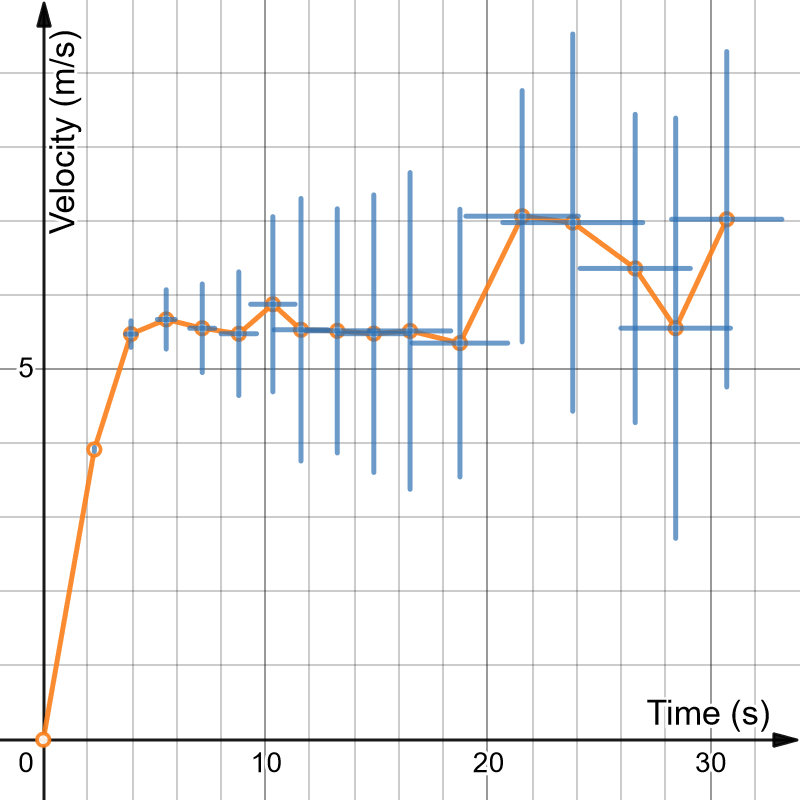
\includegraphics[scale=0.3]{pics/velocity-time.png}
\end{figure}

\subsection*{Error bar explanation}

The horizontal error bars on the graph represents the error in time, which was calculated using standard deviation of the time values collected for each of the three trials at that distance in time. The vertical error bars on the graph represent the error in velocity. As velocity was calculated by dividing distance by time, this error value was calculated by combining the measuring error for distance (which was calculated based off the increments of the ruler used) with the error for time. See ``Sample Calculations'' above for further details.

\section{Analysis}

Velocity rose from 0 to 5 very quickly as expected, as the athlete is accelerating from rest to their full speed.

From 6 to 19 seconds, the velocity of the athlete stays almost exactly consistent at around 5.5 meters per second, as evidenced by the relatively flat slope of the athlete's speed.  There's an occasional unexplained increase in velocity at 10 seconds, which could be an error in hurdle placement.

From 19 to 22 seconds, there is a huge perceived increase in athelte speed (roughly 1.5 \(\frac{m}{s}\)). According to literature researched in the background,  \parencite{martin1997better} the creatine phosphate system should only last 15--20 seconds. There are a couple explanations for this. One, this huge increase in speed jumps in coincides with use of the perspective shift method to measure distance travelled. The error bars at this point in time are longer than \(2\frac{m}{s}\), which the data point at 28.5 seconds reaching almost \(3\frac{m}{s}\). The implication that the perspective shift method has on the data is further explored in the error section. The other two factors that can be used to explain this phoenomenon is the athlete is coming off the bend of the track. When the athlete is in the bend, they have to exert energy to turn. However, for the straight run to the end, no turning is required. This could make it so that their speed seemingly increases, as they pass hurdles sooner in the straights than the curves.

Finally, the athlete speed sharply drops off until 28 seconds, where from 30 seconds it increases sharply again as the athlete approaches the finish line. This decrease in effective speed could be evidence in support of the fact that the athlete is suffering from muscle fatigue, sharply decreasing in speed. The athlete speed increase at the end could be explained by motivation, because as the athlete nears the finish line they would be more motivated to finish.

\section{Conclusion}

In conclusion, the data partially supported the initial hypothesis that athlete velocity would decrease at an increasing rate as time went on and muscle, though not at the expected time period of 10--20 seconds. Though, this conclusion is incredibly inconclusion

\subsection{Evaluating Procedures and Future Research}

The data was not very reliable. This was because for one, the physical attributes of the contestants lead to large variations in time per meter. Second, the measuring method used for 100 meters onward casts a large amount of doubt onto whether or not the results measured are their true value.

The data was not very valid. There were two confounding factors that could've been eliminated systemically via the experiment, but were not considered. One was motivation, this was the extrinsic motivation of the athlete seeing the finish line. As the athlete neared the end, motivation played a large role on their increase in speed towards the finish line. As a future condition to mitigate this thing, athletes should be told to run for a specified amount of time instead of a specified distance. This would remove the observed phoenomenon of an increase in velocity at the end, and make motivation have less of an effect on the data. This will also remove the need to ask contestants not to pace themselves in the briefing, since they are not motivated by the fact that they must complete the 100m.

The other was the track environment, which started with a bend and ended with a straight. Because the athlete has to exert more force to turn than to run a straight, the data set of the first 20 seconds cannot be fairly compared to the data set of the second 20 seconds. One is measuring the force the athlete exerts to move forwards and sideways, while the other is measuring the force the athlete exerts to move forwards only. As a result, the velocity of the first 20 seconds could be lower than it actually should be. This is a hard factor to account for given the fact that there are no straight stretches of land greater than 100 meters around the school. Therefore, the whole exercise must be changed to account for this. Instead of sprinting, the experiment could be changed to an isometric, static exercise, such as measuring the force of a maximal handgrip \parencite{kurosawaCreatineSupplementationEnhances2003}.

Finally, another weakness was the method of interpolation used in the experiment to measure athlete distance after 100 meters, which suffered greatly from random error. By the nature of the track, as the athlete runs further away from the 100 meter point, they become smaller, and so each pixel of the image represents a greater area and thus the error becomes larger. To account for this, at the very least, the camera should be kept still at the same position for each contestant for distances after 100 meters, which would remove both the error and the manual effort required to mark different pixels for each contestant. Better yet, this method of interpolation could be scrapped altogether, instead a camera could be attached to each contestants' back, so as they pass a hurdle they are directly next to it and so there is no need to account for camera perspective.

\newpage

\raggedright{}
\printbibliography[heading=bibintoc]

\section{Appendix}

\subsection{Code for Homography Transformation}

The full code for homography transformation can be found at \href{https://github.com/SpicyRicecaker/homography}{\nolinkurl{https://github.com/SpicyRicecaker/homography}}

\subsection{Debriefing}
I'll be standing in the middle of the field. You'll get into the starting position at the 200m starting line (point to line) in a standing position. At this point, I'll start filming the video. I'll both verbally say ``ready when you are'' and raise my hand up when I'm ready for you to start. Then, whenever you feel like you're ready, run as hard as you can from the starting line to the finish line (point to the finish line).

\newpage

\subsection{Par-Q}

\begin{table}[H]
    \centering
    % the X in tabularx expands cell to fill
    % >{} applies command to every single cell
    \begin{tabular}{@{}c|c|p{12cm}@{}} \toprule
        {Yes} & {No} & {Question}                                                                                                                       \\ \midrule
              &      & Has your doctor ever said that you have a heart condition and that you should only do physical activity recommended by a doctor? \\ \hline
              &      & Do you feel pain in your chest when you do physical activity?                                                                    \\ \hline
              &      & In the past month, have you had chest pain when you were not doing physical activity?                                            \\ \hline
              &      & Do you lose your balance because of dizziness or do you ever lose consciousness?                                                 \\ \hline
              &      & Do you have a bone or joint problem that could be made worse by a change in your physical activity?                              \\ \hline
              &      & Is your doctor currently prescribing drugs (for example, water pills) for your blood pressure or heart condition?                \\ \hline
              &      & Do you know of any other reason why you should not do physical activity?
    \end{tabular}
\end{table}

``I have read, understood and completed this questionnaire. Any questions I had were answered to my full satisfaction.''

Signature:
\noindent\rule{0.8\textwidth}{1pt}

\end{document}